\documentclass[12pt]{article}

\usepackage{amsmath}
\usepackage{amssymb}
\usepackage[dvips]{graphicx}
%\usepackage{lscape}
\usepackage{eepic}
\usepackage{color}
\usepackage{wasysym} % \female \male
\usepackage[landscape,pdftex]{geometry}
\usepackage{fancyhdr}
\usepackage{hyperref}

\definecolor{cantelope}{rgb}{1.0,0.8,0.4}
\hypersetup{
    colorlinks, urlcolor={cantelope}
}
\hypersetup{pdfpagemode=UseNone} % don't show bookmarks on initial view

\DeclareOption{bigsym}{\DeclareSymbolFont{largesymbols}{OMX}{psycm}{m}{n}}
\ProcessOptions

\setlength{\oddsidemargin}{-0.75in}
\setlength{\evensidemargin}{-0.75in}
\setlength{\topmargin}{-1in}
\setlength{\textheight}{7.75in}
\setlength{\textwidth}{10.5in}
\setlength{\footskip}{0in}
\setlength{\parindent}{0pt}
\setlength{\rightskip}{0pt plus 1fil} % makes ragged right

\renewcommand{\familydefault}{phv} % helvetica

% following: color
\definecolor{mybgcolor}{rgb}{0,0,0.3125}
\definecolor{myyellow}{rgb}{1,1,0.4}
\definecolor{myblue}{rgb}{0.4,0.8,1}
\definecolor{mypink}{rgb}{1,0.4,1}
\definecolor{mywhite}{rgb}{1,1,1}

% following: B/W
%\definecolor{mybgcolor}{rgb}{1,1,1}
%\definecolor{myyellow}{rgb}{0,0,0}
%\definecolor{myblue}{rgb}{0,0,0}
%\definecolor{mypink}{rgb}{0,0,0}
%\definecolor{mywhite}{rgb}{0,0,0}

% header/footer layout
\pagestyle{fancy}
\lhead{} \chead{} \rhead{}
\lfoot{} \cfoot{} \rfoot{\color{myyellow} \thepage}
\renewcommand{\headrulewidth}{0pt}
\renewcommand{\footrulewidth}{0pt}

% font sizes
\newcommand{\superlarge}{\fontsize{60}{60} \selectfont}
\newcommand{\titlesize}{\fontsize{40}{50} \selectfont}
\newcommand{\headsize}{\fontsize{35}{35} \selectfont}
\newcommand{\textsize}{\fontsize{30}{35} \selectfont}
\newcommand{\smallsize}{\fontsize{25}{30} \selectfont}
\newcommand{\smallersize}{\fontsize{20}{25} \selectfont}
\newcommand{\smallestsize}{\fontsize{18}{22} \selectfont}
\newcommand{\lod}{\text{LOD}}
\newcommand{\rss}{\text{RSS}}
\newcommand{\var}{\text{var}}
\newcommand{\M}{\text{M}}
%\renewcommand{\log}{\text{log}}
%\renewcommand{\max}{\text{max}}



\pagecolor{mybgcolor}
\color{mywhite}

\begin{document}
\thispagestyle{empty}

\begin{center}
\titlesize \color{myyellow}


\vspace*{15mm}

QTL mapping 4: multivariate phenotypes

\color{mypink}
\rule{10in}{1mm}
%\vspace{-10mm}

\vspace{5mm}

\textsize \color{myblue}
Karl Broman
\vspace{5mm}

\color{mywhite}
{\smallsize Biostatistics and Medical Informatics

University of Wisconsin -- Madison
\vspace{20mm}


\href{http://kbroman.org}{\tt kbroman.org} \\[3pt]
\href{https://github.com/kbroman}{\tt github.com/kbroman} \\
\href{https://twitter.com/kwbroman}{\tt @kwbroman}
}

\end{center}



\newpage

\headsize \color{myyellow}
\hfill \begin{minipage}{5.75in}
\centering
Why multiple phenotypes?
\end{minipage}

\vspace{30mm}

\color{mywhite} \smallsize

\hspace*{0.5in}
\begin{minipage}[t]{9.5in}
  \begin{itemize}
    \itemsep12pt
  \item Might as well measure a bunch of stuff
  \item Not quite sure what to measure
  \item Interested in several related features
  \item Trying to get at intermediate biochemical processes
  \item What happens over time?
  \item Reduced measurement error $\rightarrow$ greater power
  \end{itemize}
\end{minipage}

\newpage

\headsize \color{myyellow}
\hfill \begin{minipage}{5.75in}
\centering
Goals
\end{minipage}

\vspace{30mm}

\color{mywhite} \smallsize

\hspace*{0.5in}
\begin{minipage}[t]{9.5in}
  \begin{itemize}
    \itemsep18pt
  \item Use multiple phenotypes to improve QTL detection
  \item Do traits share QTL (pleiotropy)?
  \item Causal relationships among traits?
  \item Effects of QTL across time
  \end{itemize}
\end{minipage}



\newpage

\headsize \color{myyellow}
\hfill \begin{minipage}{5.75in}
\centering
Pleiotropy?
\end{minipage}

\vspace{20mm}

\centerline{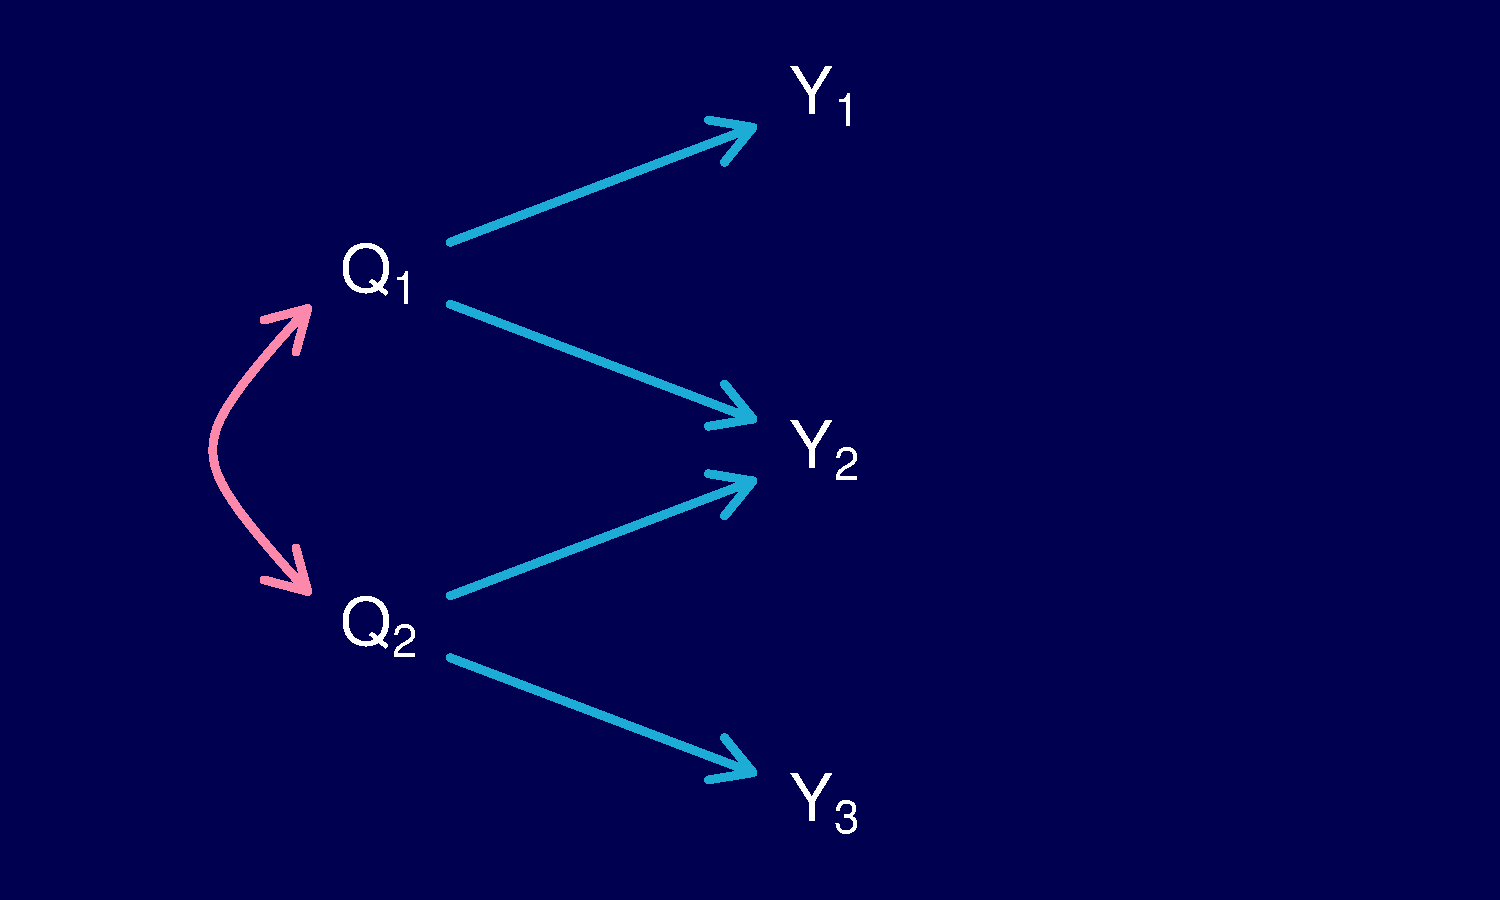
\includegraphics{Figs/pleiotropy_network.pdf}}


\newpage

\headsize \color{myyellow}
\hfill \begin{minipage}{5.75in}
\centering
Causal?
\end{minipage}

\vspace{22.3mm}

\centerline{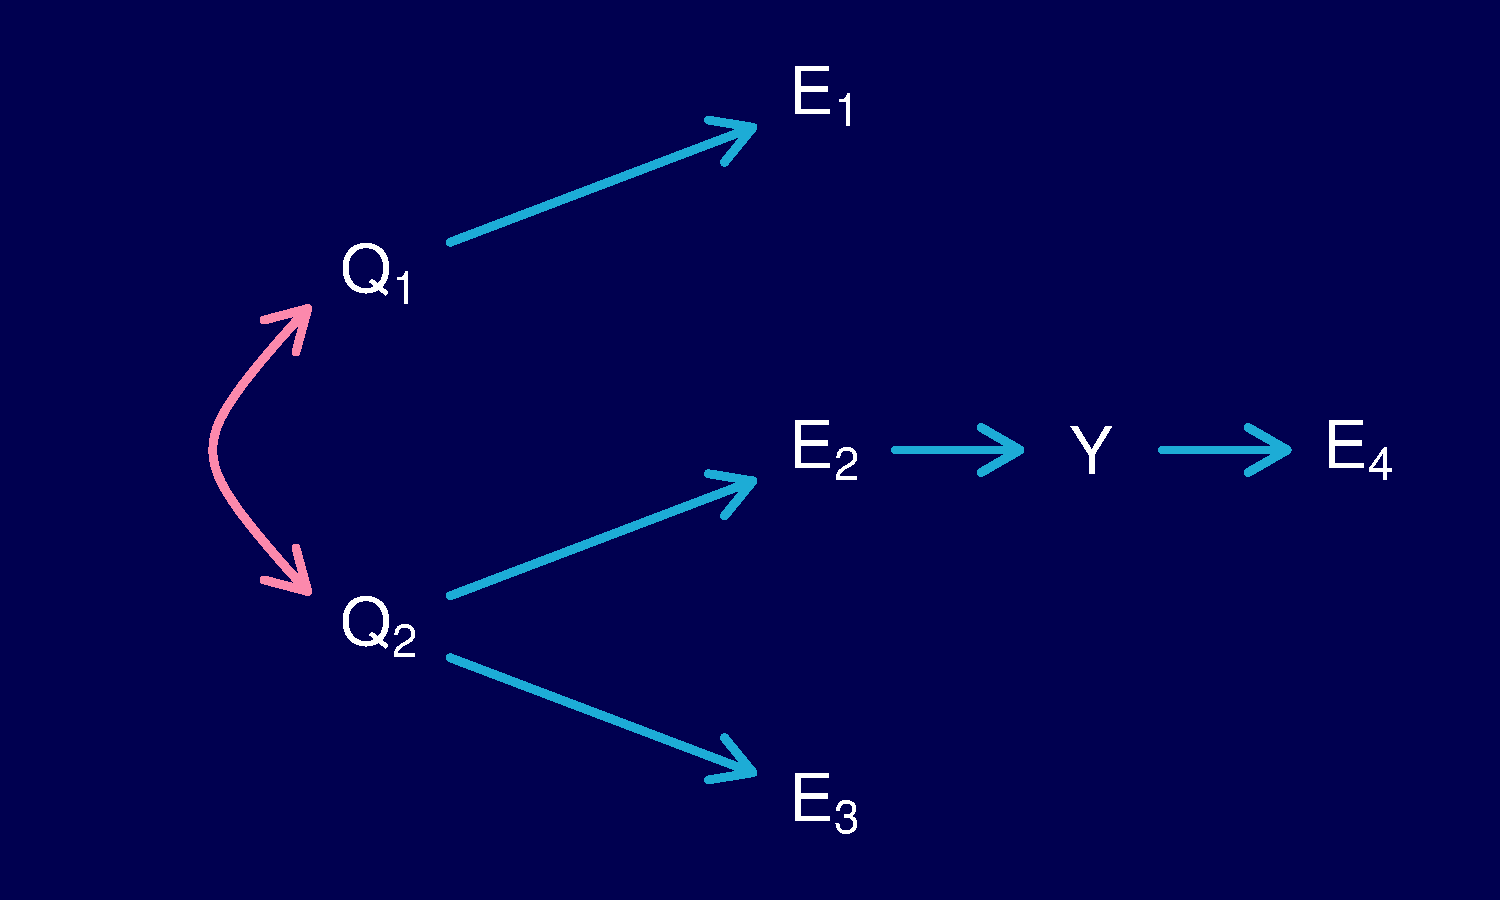
\includegraphics{Figs/causal_network.pdf}}



\newpage

\addtocounter{page}{-1}


\headsize \color{myyellow}
\hfill \begin{minipage}{5.75in}
\centering
Basic model
\end{minipage}

\vspace{25mm}

\color{white} \smallsize

One trait:

\vspace{-18pt}

{\color{myblue} $$ y = X \beta + \epsilon, \qquad \epsilon \sim \text{N}(0, \sigma^2) $$}

\vspace{-8pt}

{\color{mybgcolor} $$ \text{LOD} = (n/2) \log_{10} ( \text{RSS}_0 /
  \text{RSS}_1 ) $$ }

\vspace{15mm}

Multiple traits:

\vspace{-18pt}

{\color{myblue} $$ {\color{mypink} Y} = X {\color{mypink}
    \boldsymbol{\beta}} + {\color{mypink} \boldsymbol{\epsilon}},
  \qquad \epsilon \sim \text{\color{mypink} MVN}(0, {\color{mypink} \Sigma}) $$ }

\vspace{-8pt}

{\color{mybgcolor} $$ \text{LOD} = (n/2) \log_{10} ( {|\hat{\Sigma}_0|} /
  { |\hat{\Sigma}_1|}) $$ }

\newpage

\headsize \color{myyellow}
\hfill \begin{minipage}{5.75in}
\centering
Basic model
\end{minipage}

\vspace{25mm}

\color{white} \smallsize

One trait:

\vspace{-18pt}

{\color{myblue} $$ y = X \beta + \epsilon, \qquad \epsilon \sim \text{N}(0, \sigma^2) $$}

\vspace{-8pt}

{\color{myblue} $$ \text{LOD} = (n/2) \log_{10} ( \text{RSS}_0 /
  \text{RSS}_1 ) $$ }

\vspace{15mm}

Multiple traits:

\vspace{-18pt}

{\color{myblue} $$ {\color{mypink} Y} = X {\color{mypink}
    \boldsymbol{\beta}} + {\color{mypink} \boldsymbol{\epsilon}},
  \qquad \epsilon \sim \text{\color{mypink} MVN}(0, {\color{mypink} \Sigma}) $$ }

\vspace{-8pt}

{\color{myblue} $$ \text{LOD} = (n/2) \log_{10} ( {\color{mypink} |\hat{\Sigma}_0|} /
  {\color{mypink} |\hat{\Sigma}_1|}) $$ }



\newpage

\headsize \color{myyellow}
\hfill \begin{minipage}{5.75in}
\centering
Pleiotropy?
\end{minipage}

\vspace{25mm}

\color{mywhite} \smallersize

\hspace{0.5in} \begin{minipage}{9.5in}

  \begin{itemize}
    \itemsep18pt

  \item Consider two traits
  \item Assume each affected by a single QTL
  \item Scan chromosome for single QTL, assuming it affects both
  \item Two-dimensional scan over chromosome, one QTL affecting one
    trait and other affecting the other trait
  \item Significance?
    {\color{myblue}
    \begin{itemize}
    \item Parametric bootstrap using fitted single-QTL model
    \item Stratified permutation test, permuting within strata
      defined by genotype at estimated single QTL
      \end{itemize} }

  \end{itemize}


\end{minipage}

\newpage

\headsize \color{myyellow}
\hfill \begin{minipage}{5.75in}
\centering
Traits over time
\end{minipage}

\vspace{25mm}

\color{mywhite} \smallersize

\hspace{0.5in} \begin{minipage}{9.5in}

  \begin{itemize}
    \itemsep18pt

  \item Fit model to each curve; use parameters as phenotypes
  \item Full QTL model of curves, where parameters depend on QTL genotypes
  \item Dimension reduction $\rightarrow$ standard multivariate QTL
    analysis
  \item Treat each time point individually, and then combine LOD
    scores
  \end{itemize}

\end{minipage}


\newpage

\headsize \color{myyellow}
\hfill \begin{minipage}{5.75in}
\centering
Gough Island
\end{minipage}

\vspace{25mm}

\centerline{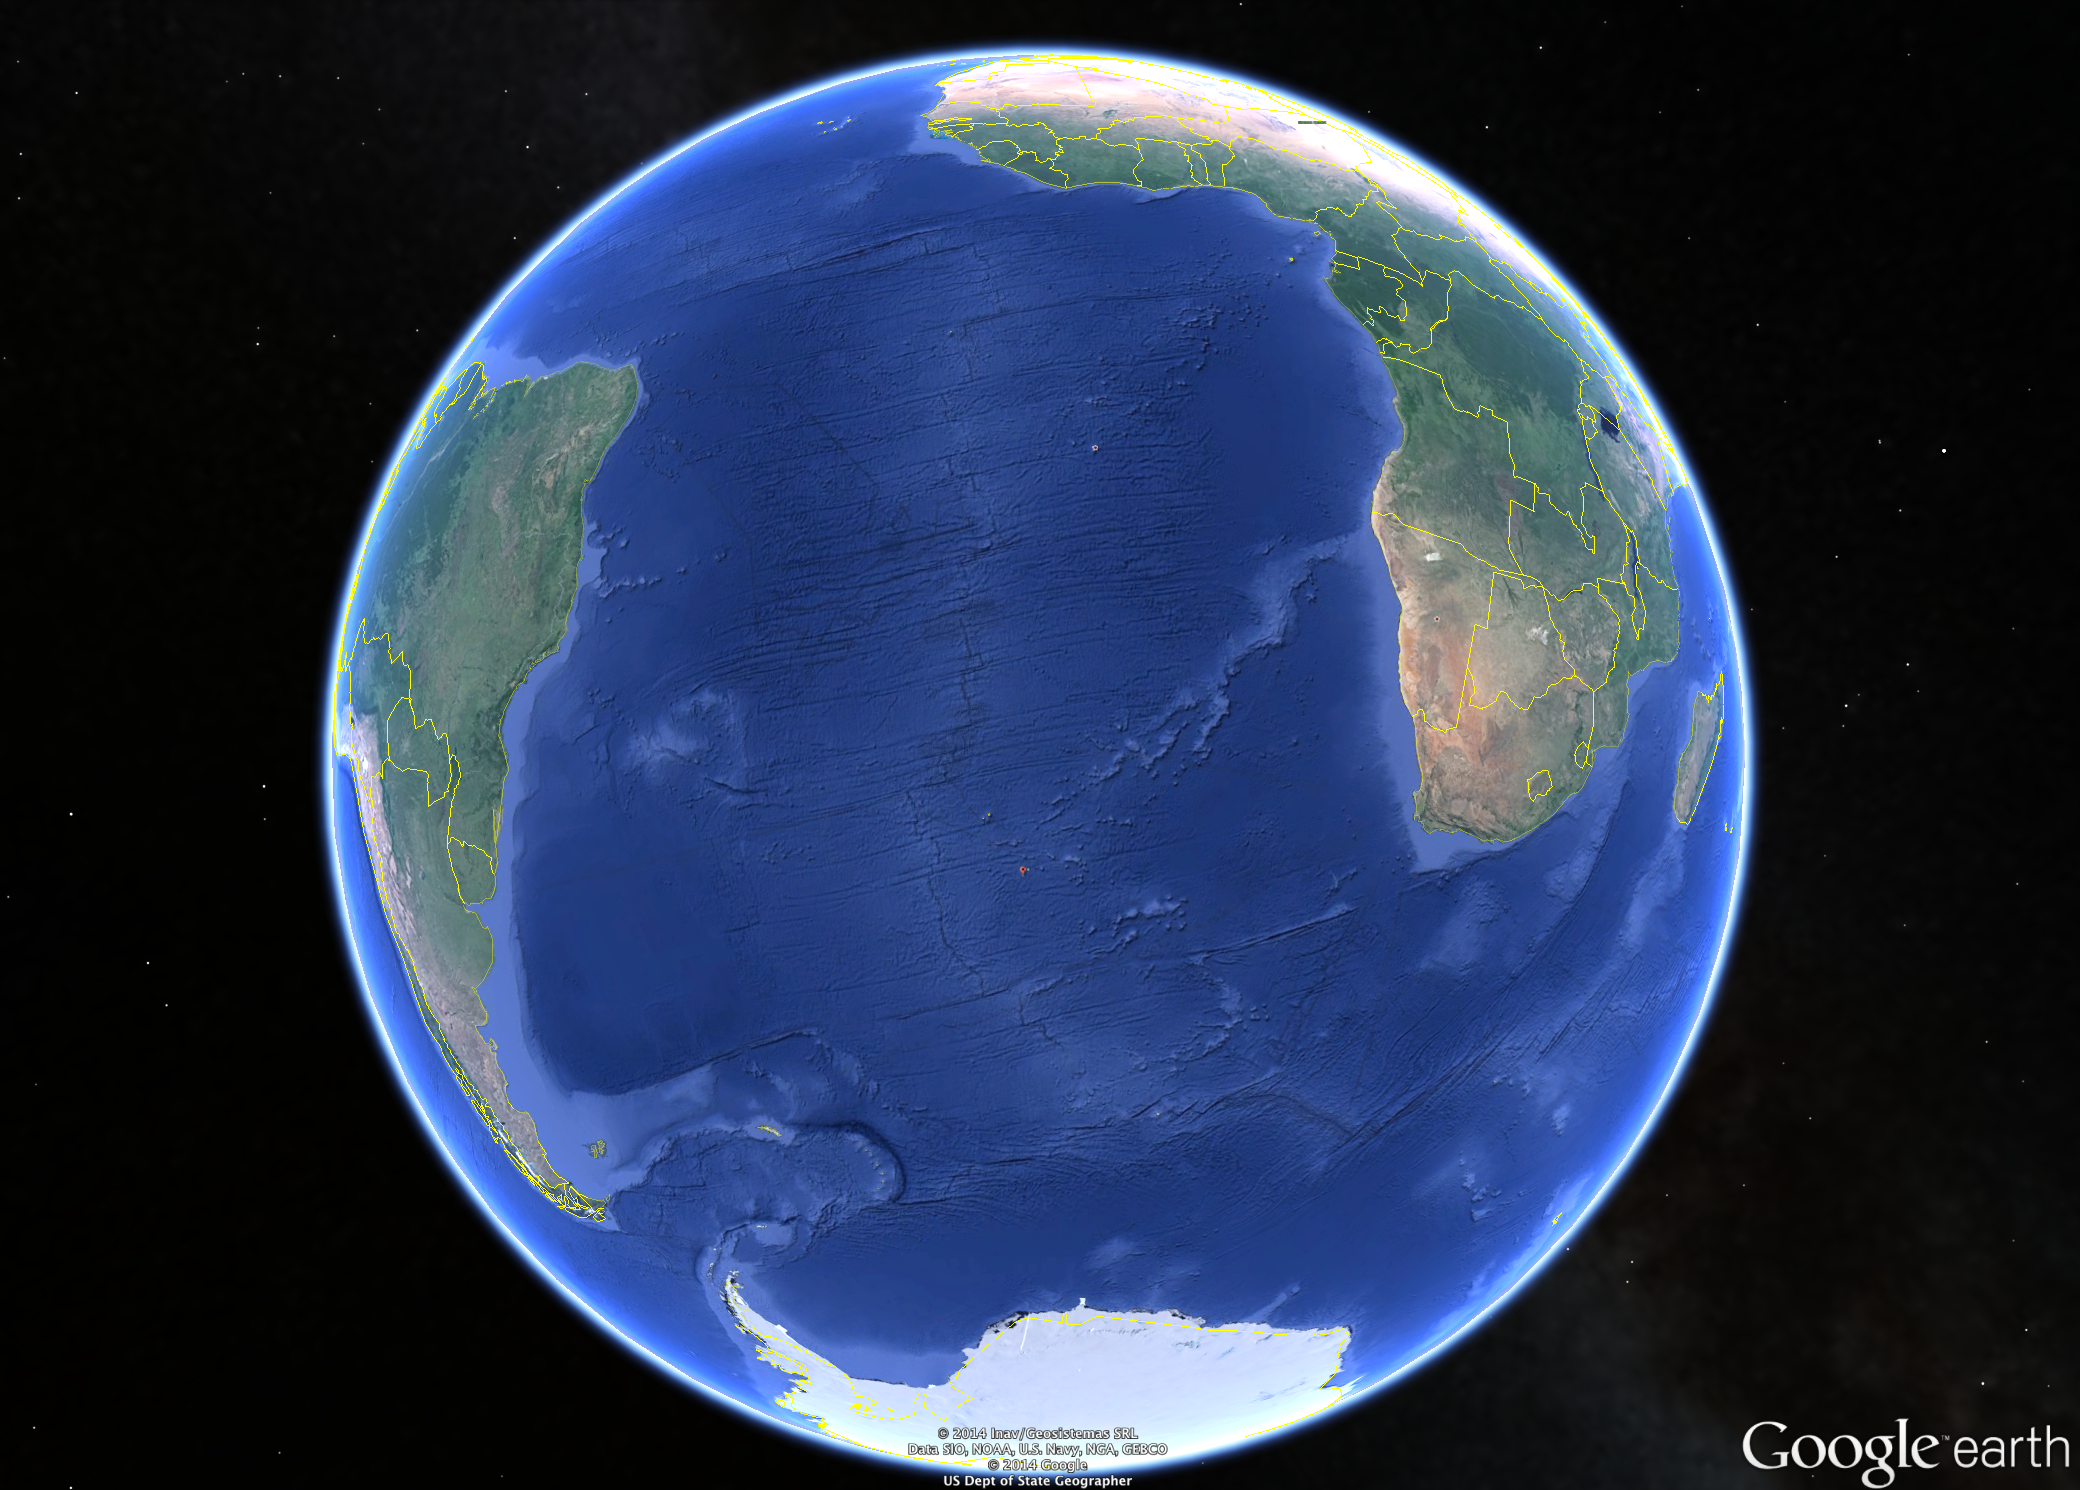
\includegraphics[height=0.8\textheight]{Figs/Gough_google_earth.png}}


\newpage

\addtocounter{page}{-1}

\headsize \color{myyellow}
\hfill \begin{minipage}{5.75in}
\centering
Gough Island
\end{minipage}

\vspace{25mm}

\centerline{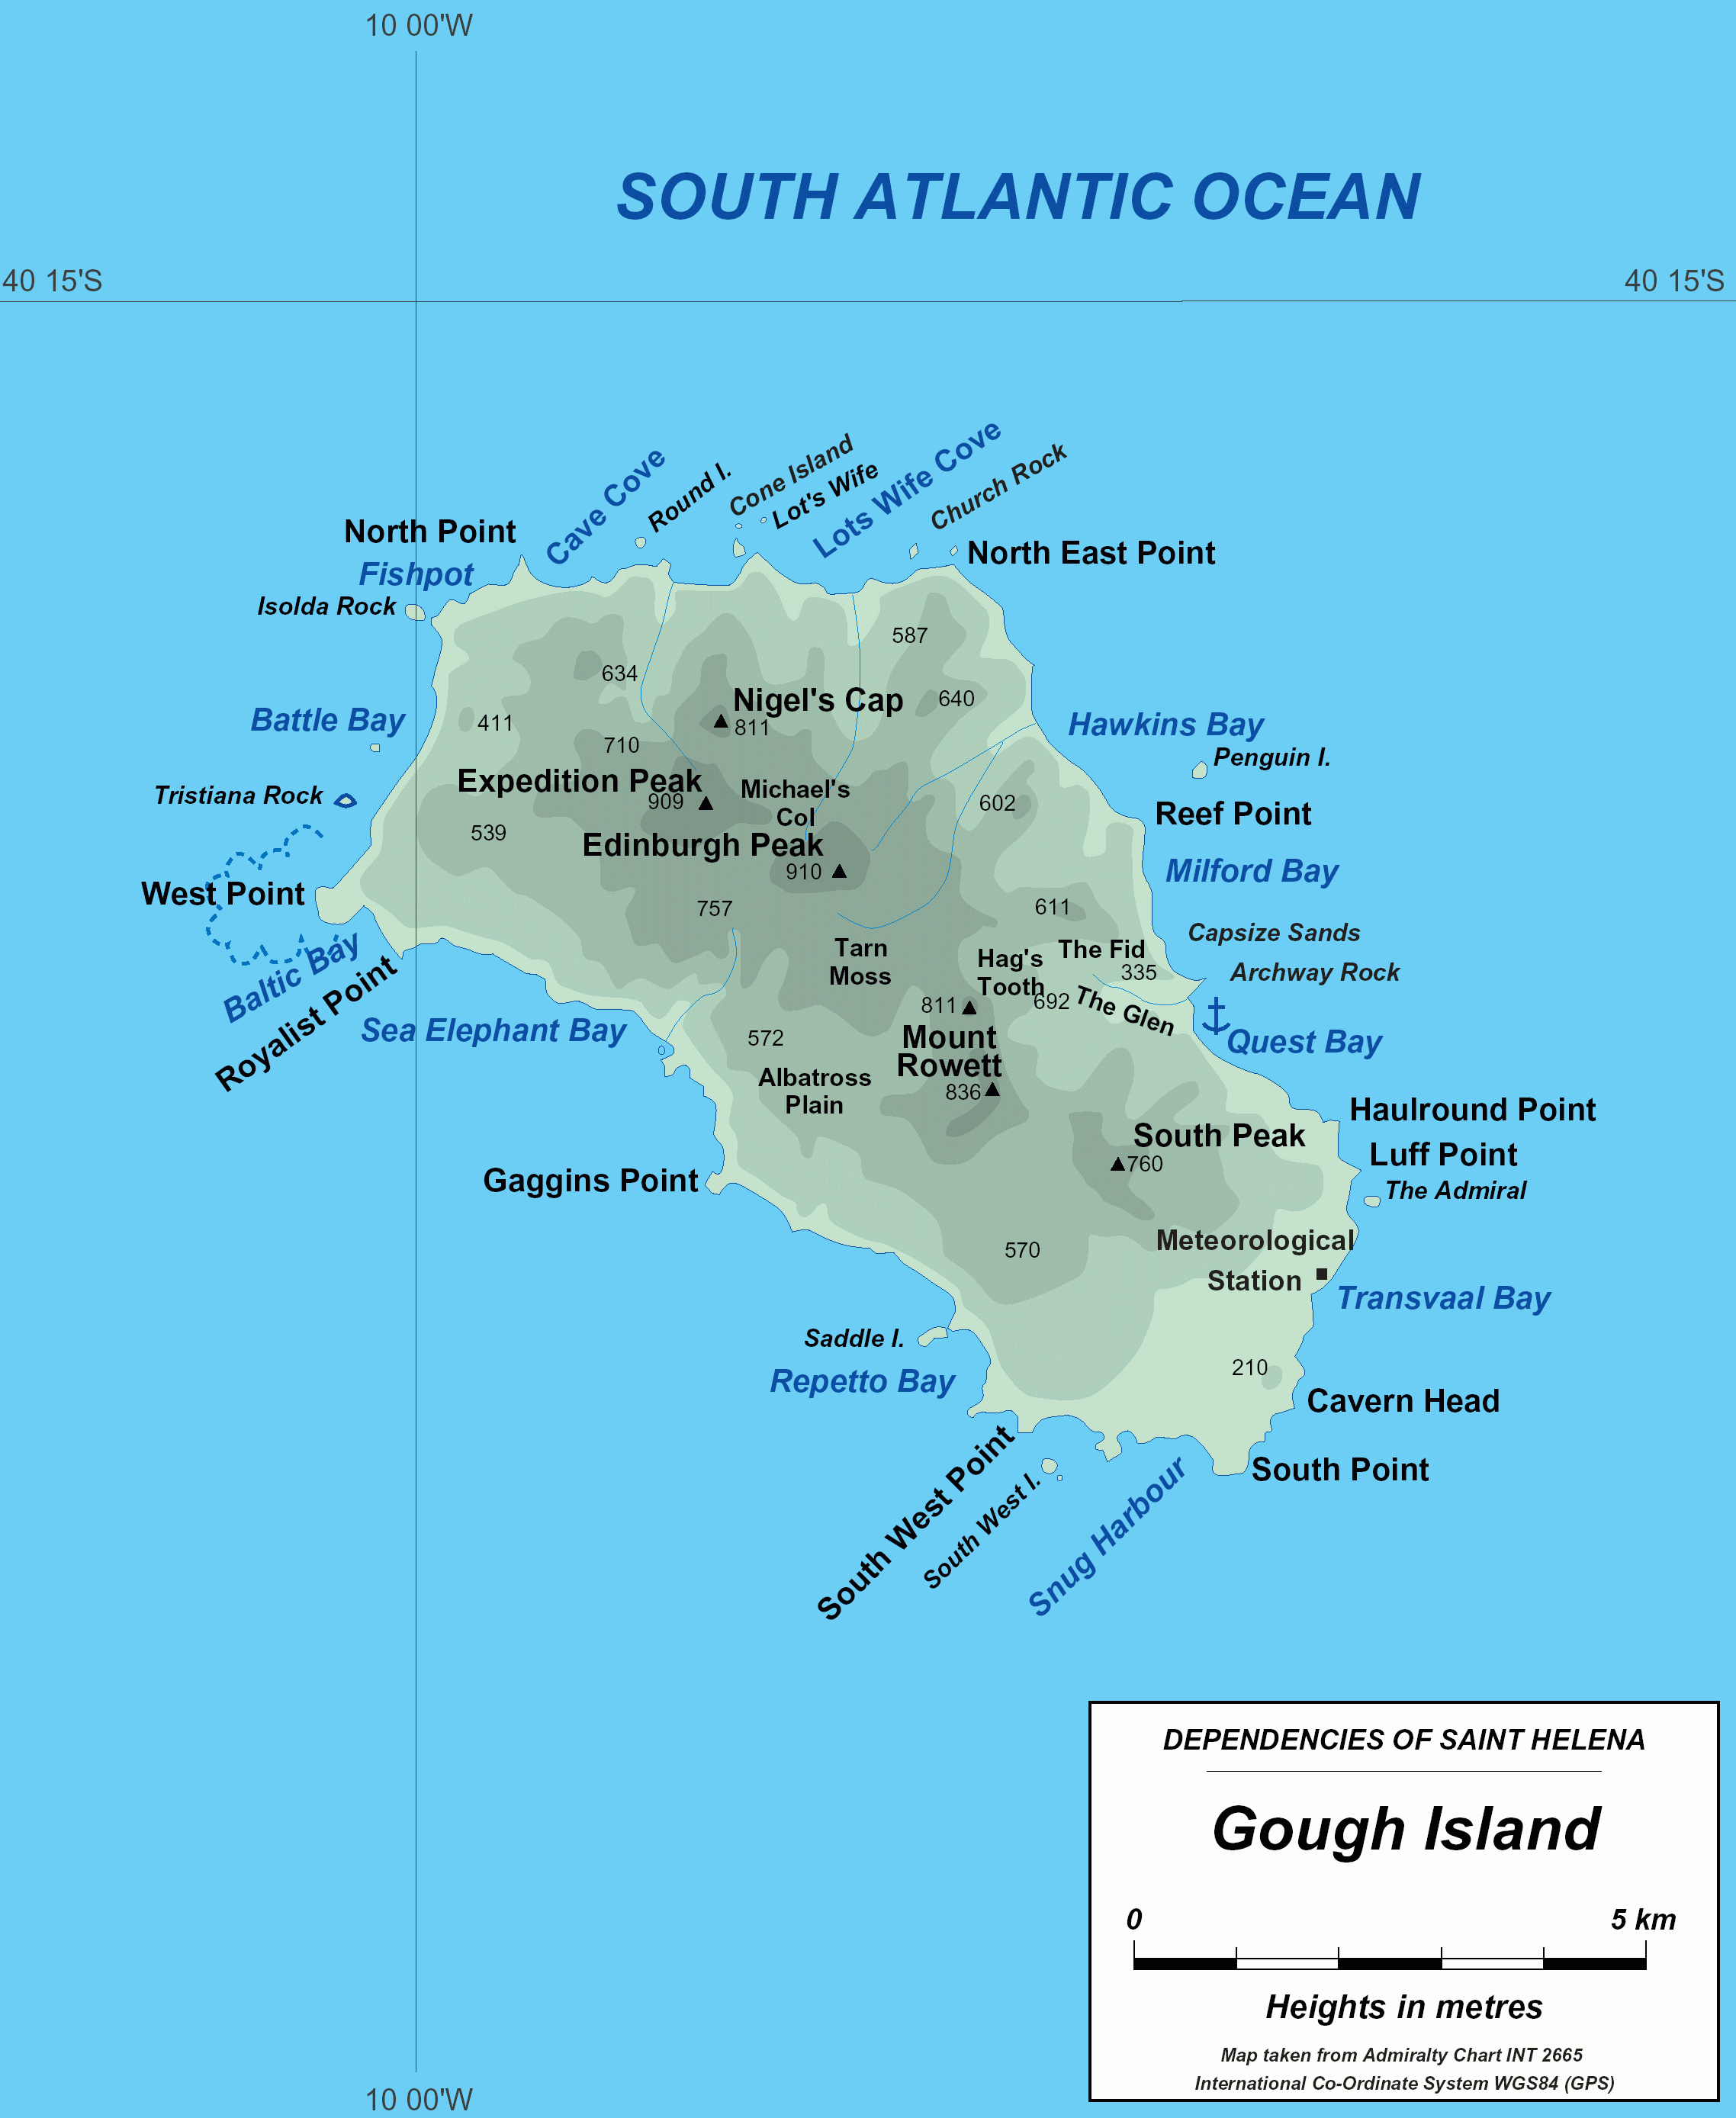
\includegraphics[height=0.8\textheight]{Figs/Gough-Island-Map.png}}


\newpage

\addtocounter{page}{-1}

\headsize \color{myyellow}
\hfill \begin{minipage}{5.75in}
\centering
Gough Island
\end{minipage}

\vspace{25mm}

\centerline{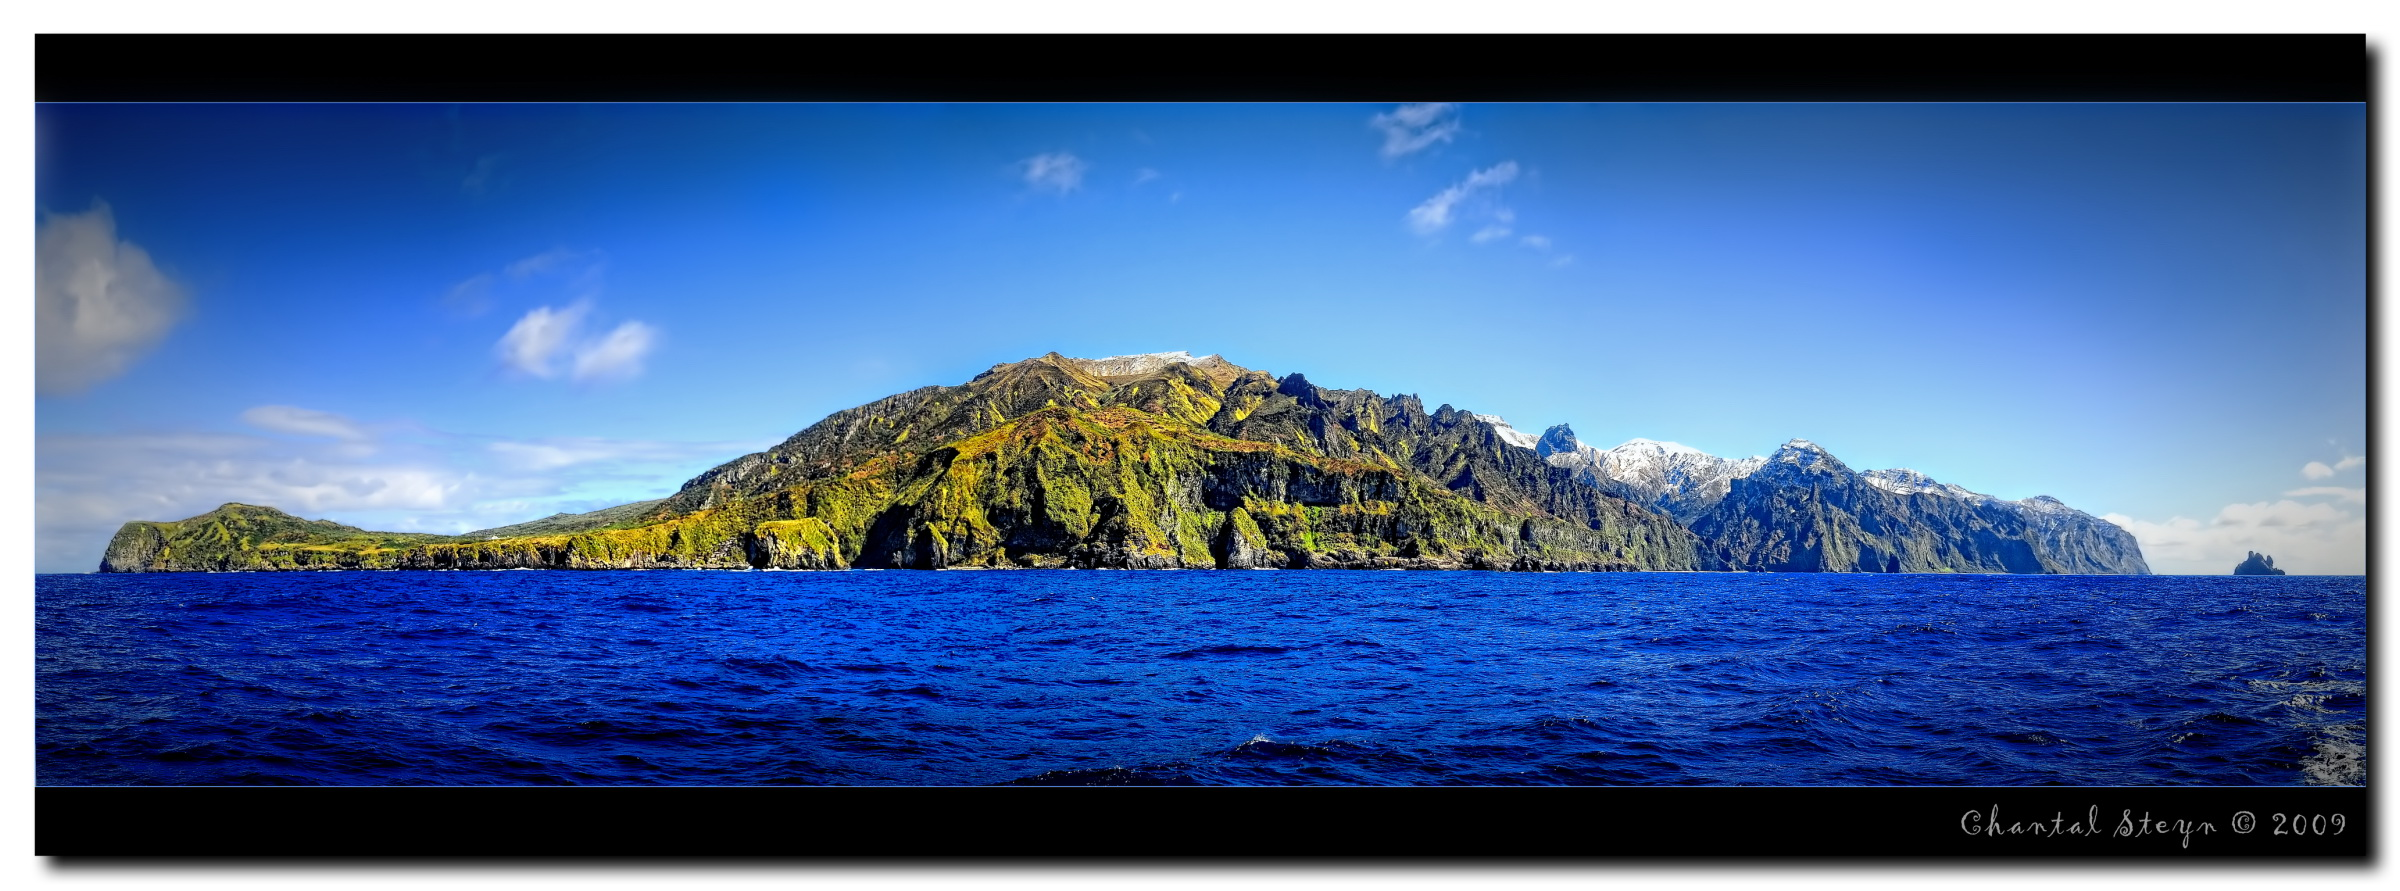
\includegraphics[width=\textwidth]{Figs/gough_wholeisland.jpg}}



\newpage

\headsize \color{myyellow}
\hfill \begin{minipage}{5.75in}
\centering
Big rodents
\end{minipage}

\vspace{10mm}

\centerline{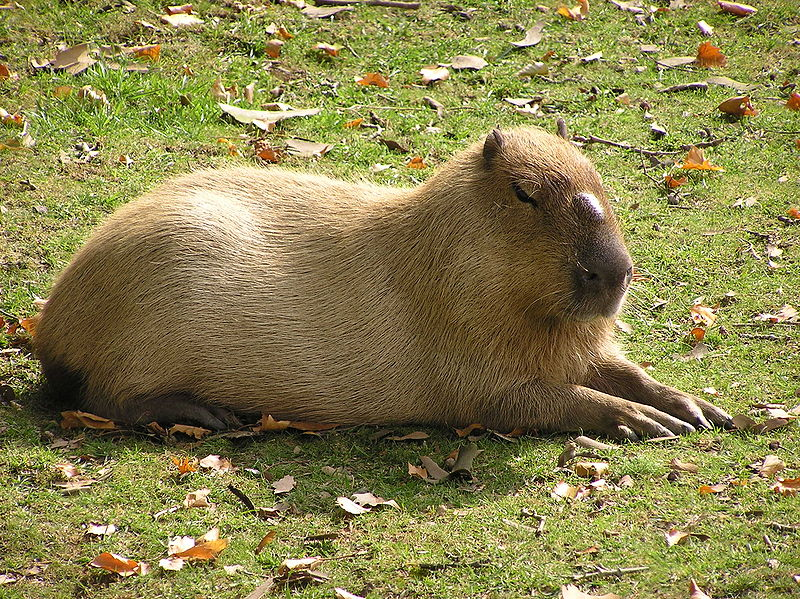
\includegraphics[width=0.8\textwidth]{Figs/capybara.jpg}}




\newpage

\addtocounter{page}{-1}

\headsize \color{myyellow}
\hfill \begin{minipage}{5.75in}
\centering
Big rodents
\end{minipage}

\vspace{10mm}

\centerline{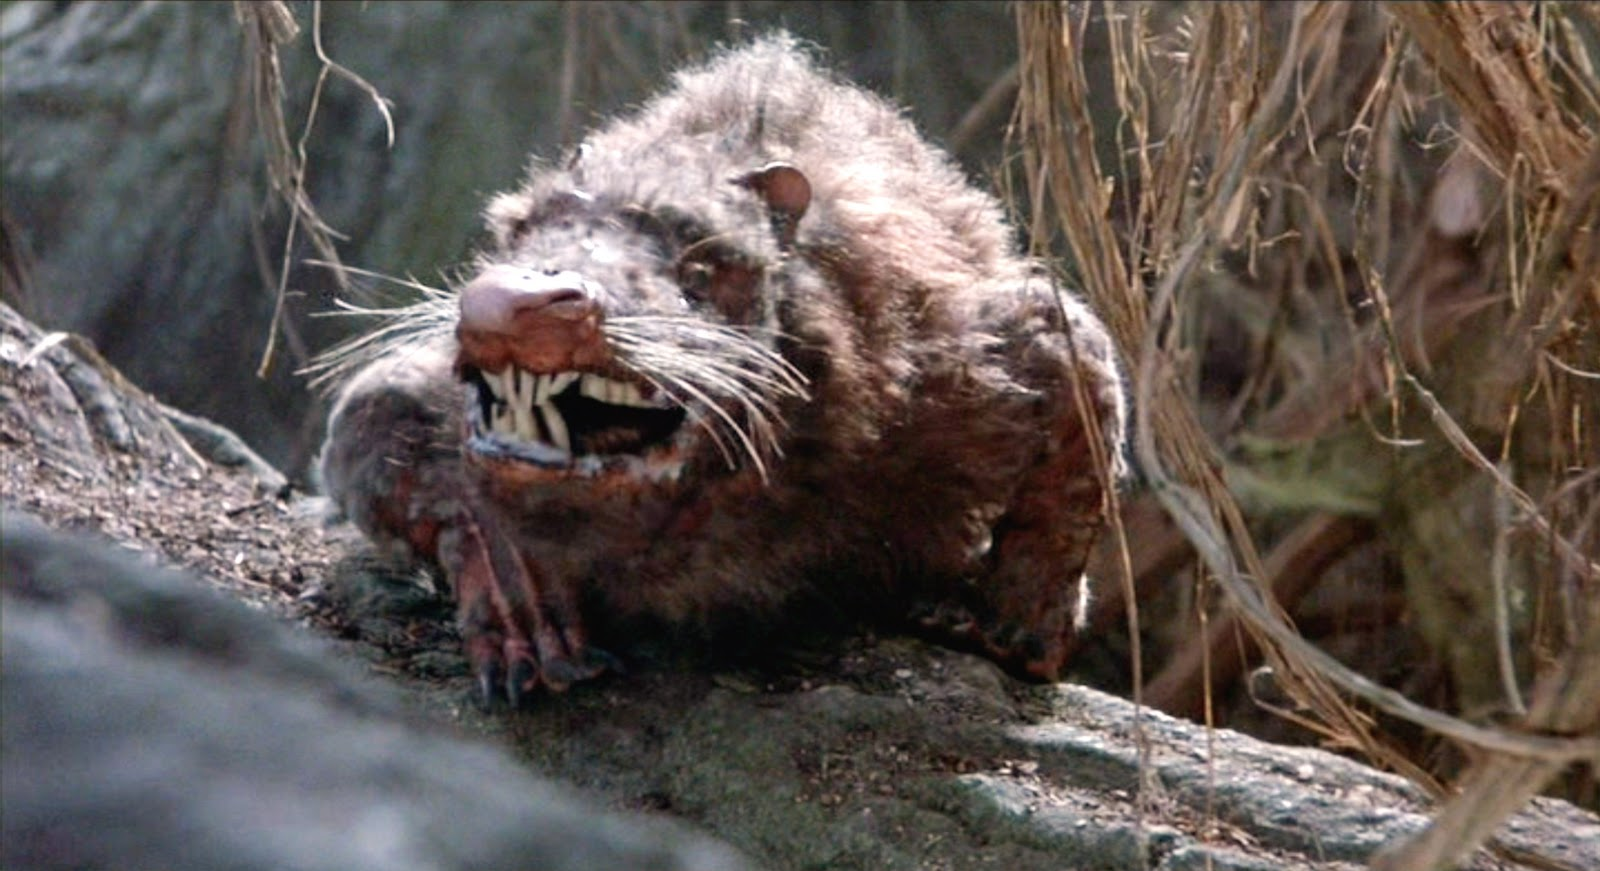
\includegraphics[width=\textwidth]{Figs/rodents_of_unusual_size.jpg}}




\newpage

\addtocounter{page}{-1}

\headsize \color{myyellow}
\hfill \begin{minipage}{5.75in}
\centering
Big rodents
\end{minipage}

\vspace{10mm}

\centerline{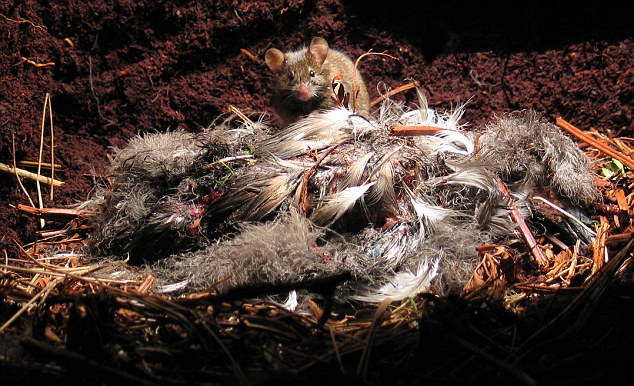
\includegraphics[width=\textwidth]{Figs/gough_mouse_with_bird.jpg}}


\newpage

\headsize \color{myyellow}
\hfill \begin{minipage}{5.75in}
\centering
WSB and Gough mice
\end{minipage}

\vspace{30mm}

\centerline{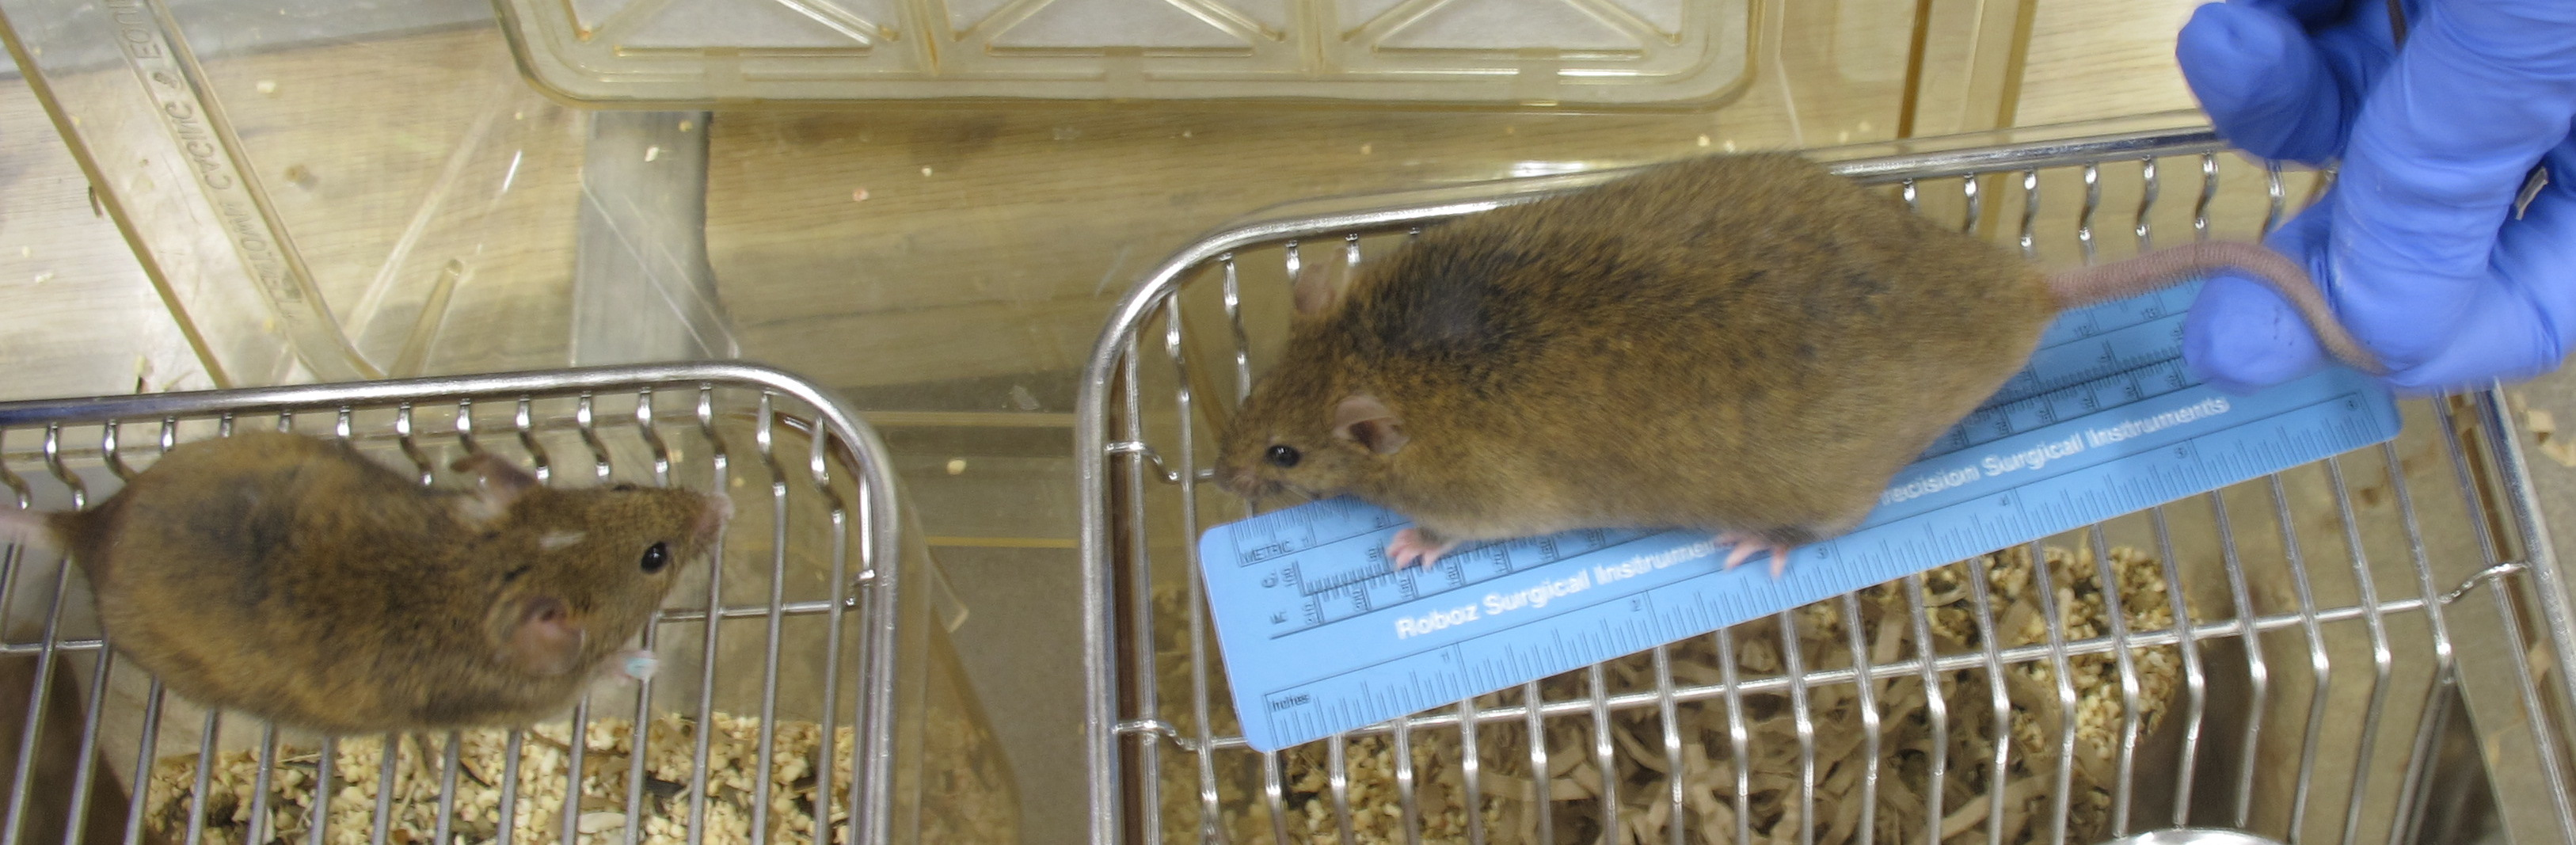
\includegraphics[width=\textwidth]{Figs/wsb_508_and_gough_535_cropped.jpg}}


\newpage

\headsize \color{myyellow}
\hfill \begin{minipage}{5.75in}
\centering
Growth curves
\end{minipage}

\vspace{30mm}

\centerline{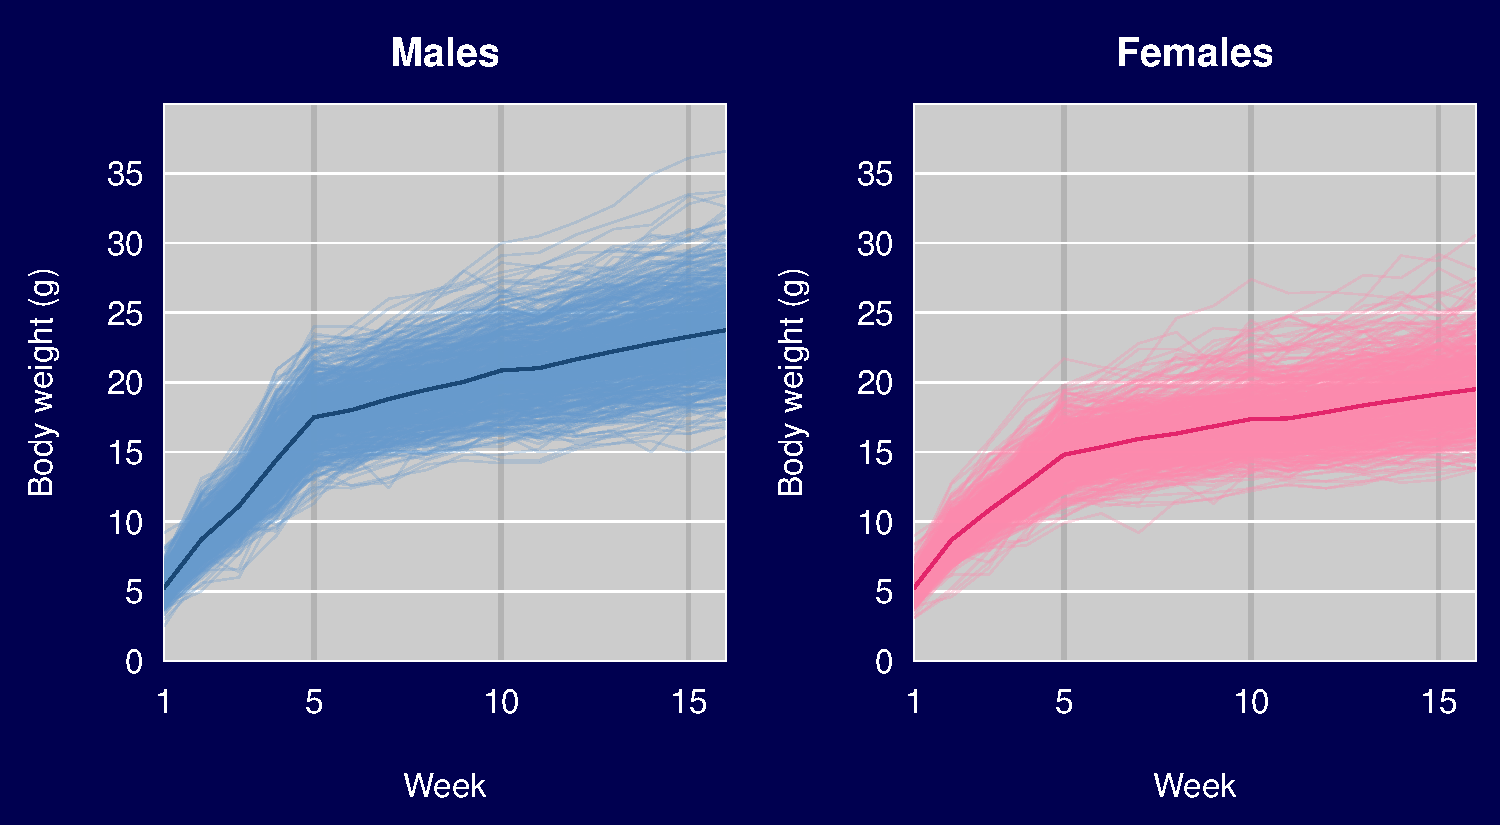
\includegraphics{Figs/growth1.pdf}}


\newpage

\addtocounter{page}{-1}

\headsize \color{myyellow}
\hfill \begin{minipage}{5.75in}
\centering
Growth curves
\end{minipage}

\vspace{30mm}

\centerline{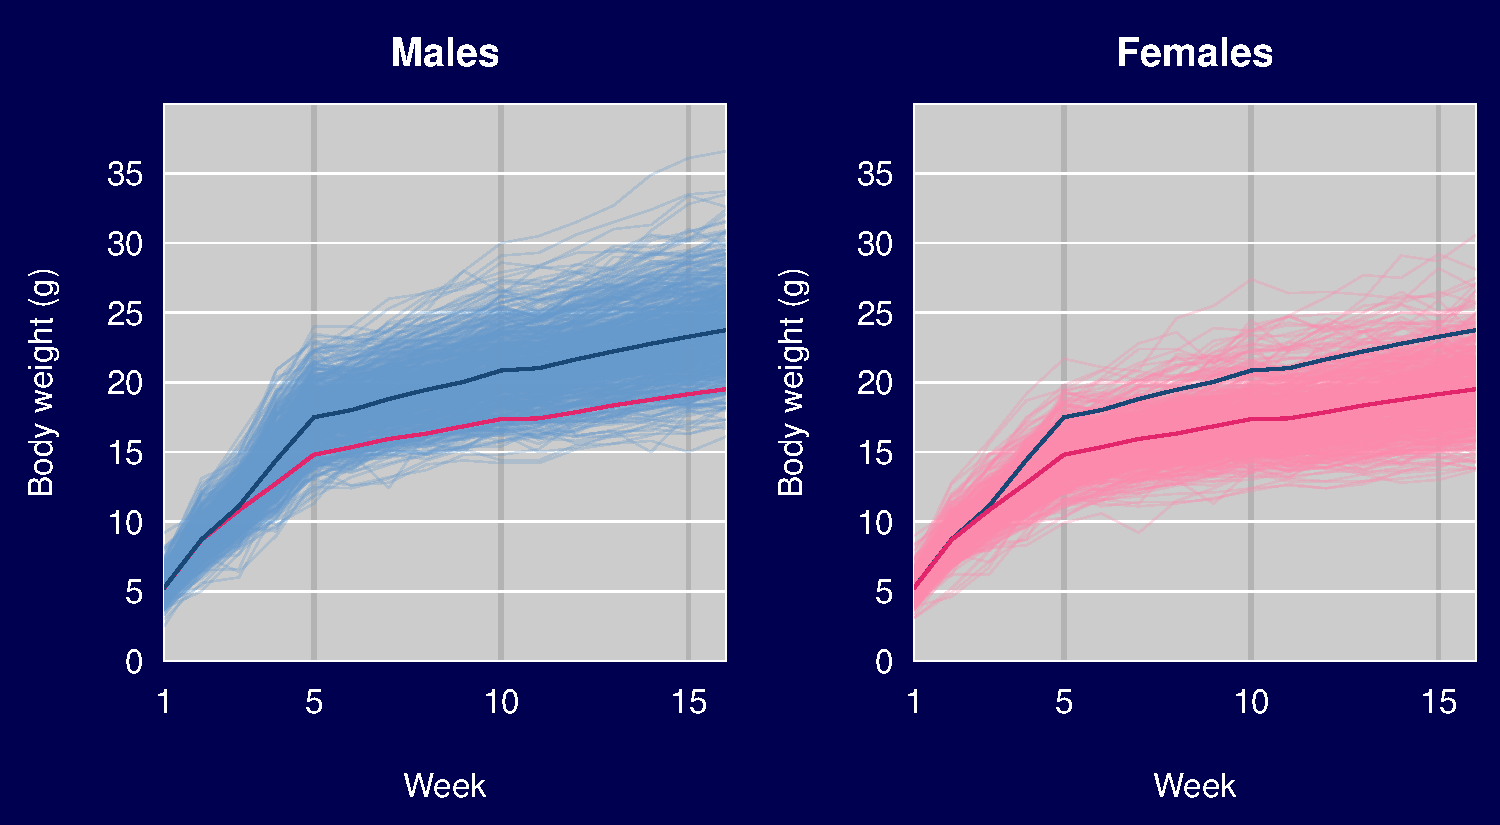
\includegraphics{Figs/growth2.pdf}}


\newpage

\addtocounter{page}{-1}

\headsize \color{myyellow}
\hfill \begin{minipage}{5.75in}
\centering
Growth curves
\end{minipage}

\vspace{30mm}

\centerline{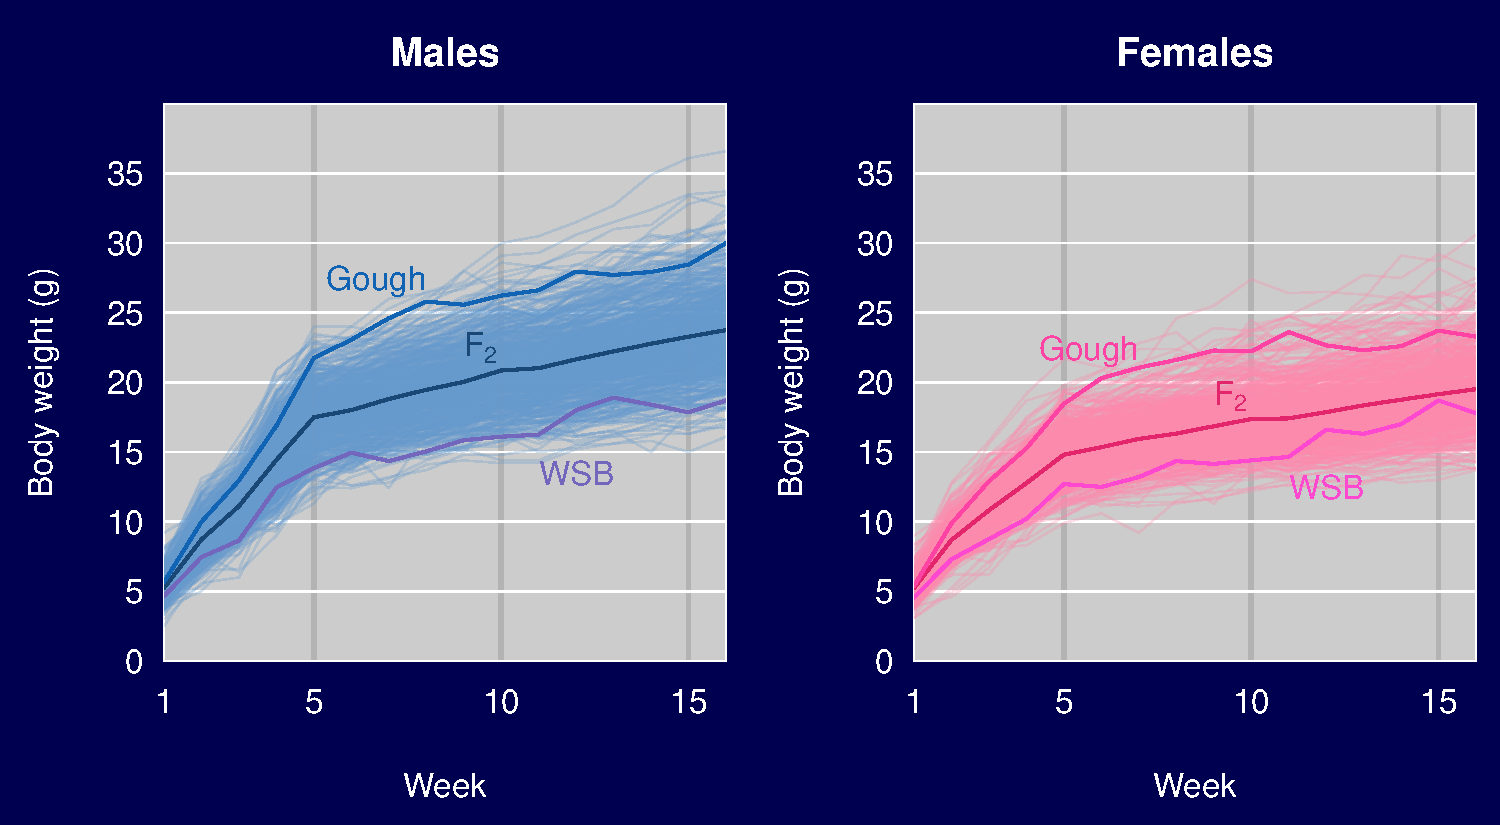
\includegraphics{Figs/growth3.pdf}}


\newpage

\headsize \color{myyellow}
\hfill \begin{minipage}{5.75in}
\centering
Growth rate
\end{minipage}

\vspace{30mm}

\centerline{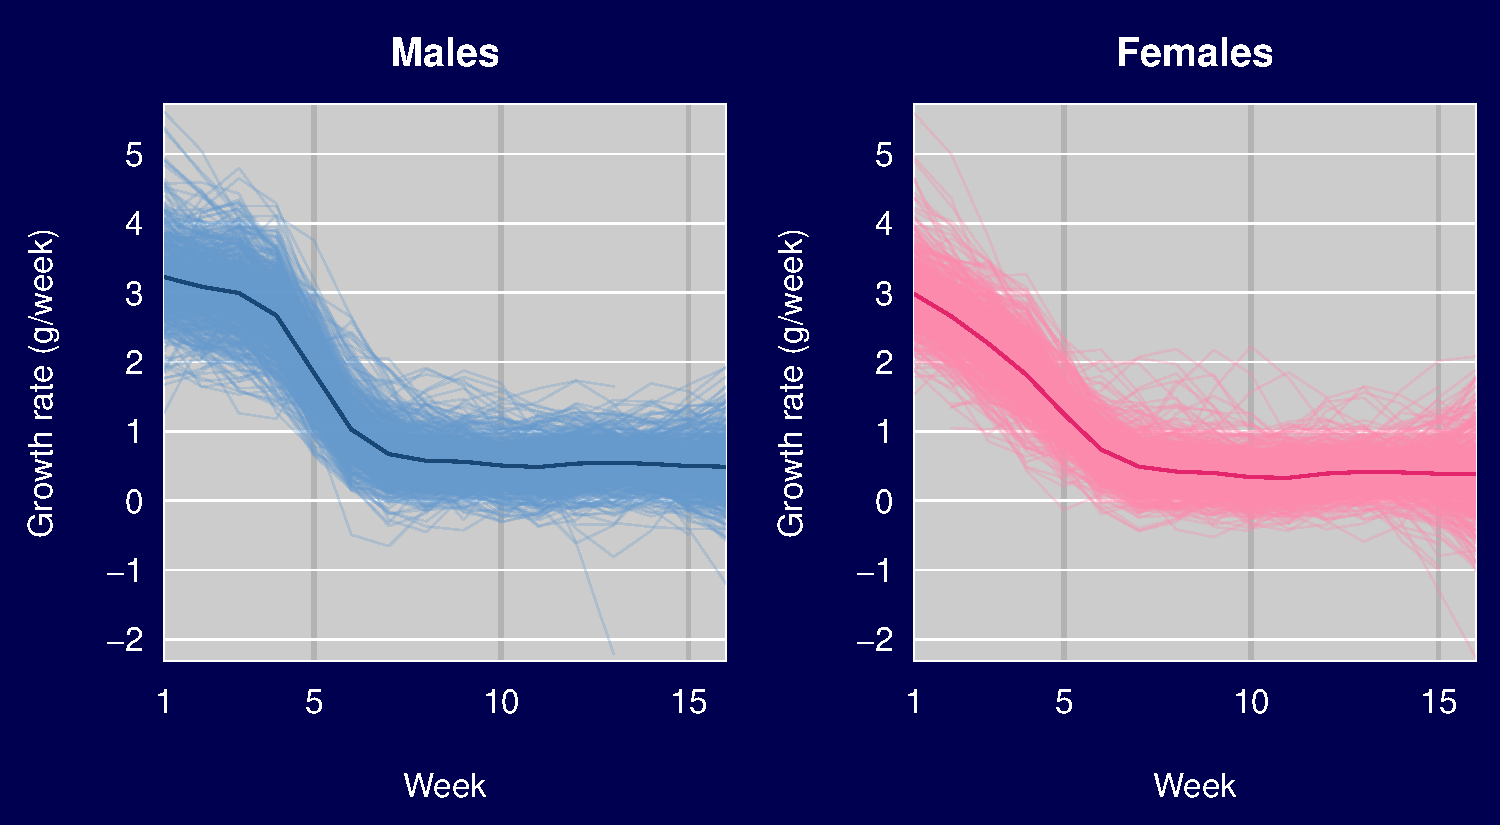
\includegraphics{Figs/rate1.pdf}}


\newpage

\addtocounter{page}{-1}

\headsize \color{myyellow}
\hfill \begin{minipage}{5.75in}
\centering
Growth rate
\end{minipage}

\vspace{30mm}

\centerline{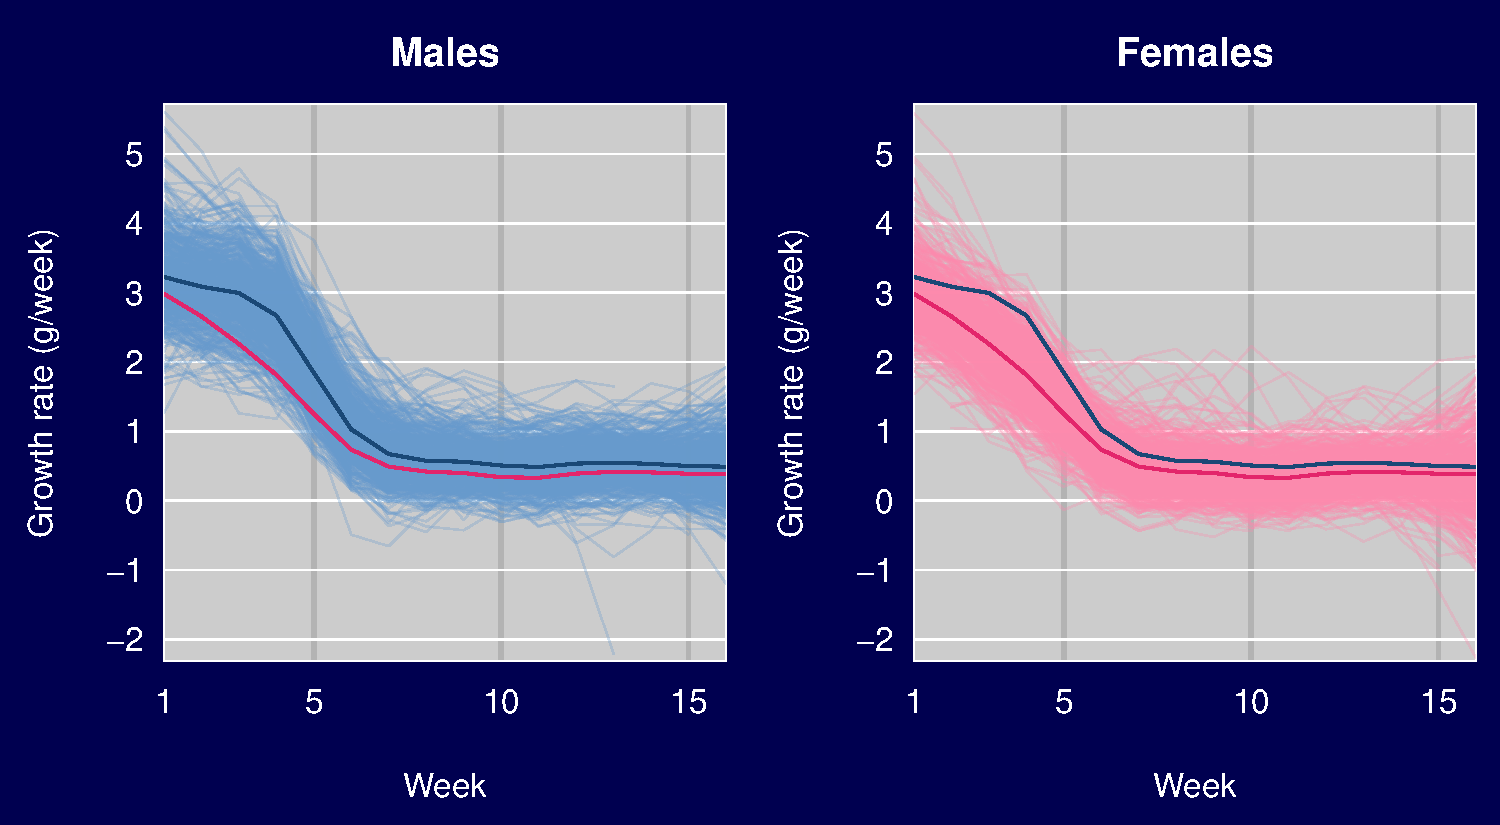
\includegraphics{Figs/rate2.pdf}}


\newpage

\addtocounter{page}{-1}

\headsize \color{myyellow}
\hfill \begin{minipage}{5.75in}
\centering
Growth rate
\end{minipage}

\vspace{30mm}

\centerline{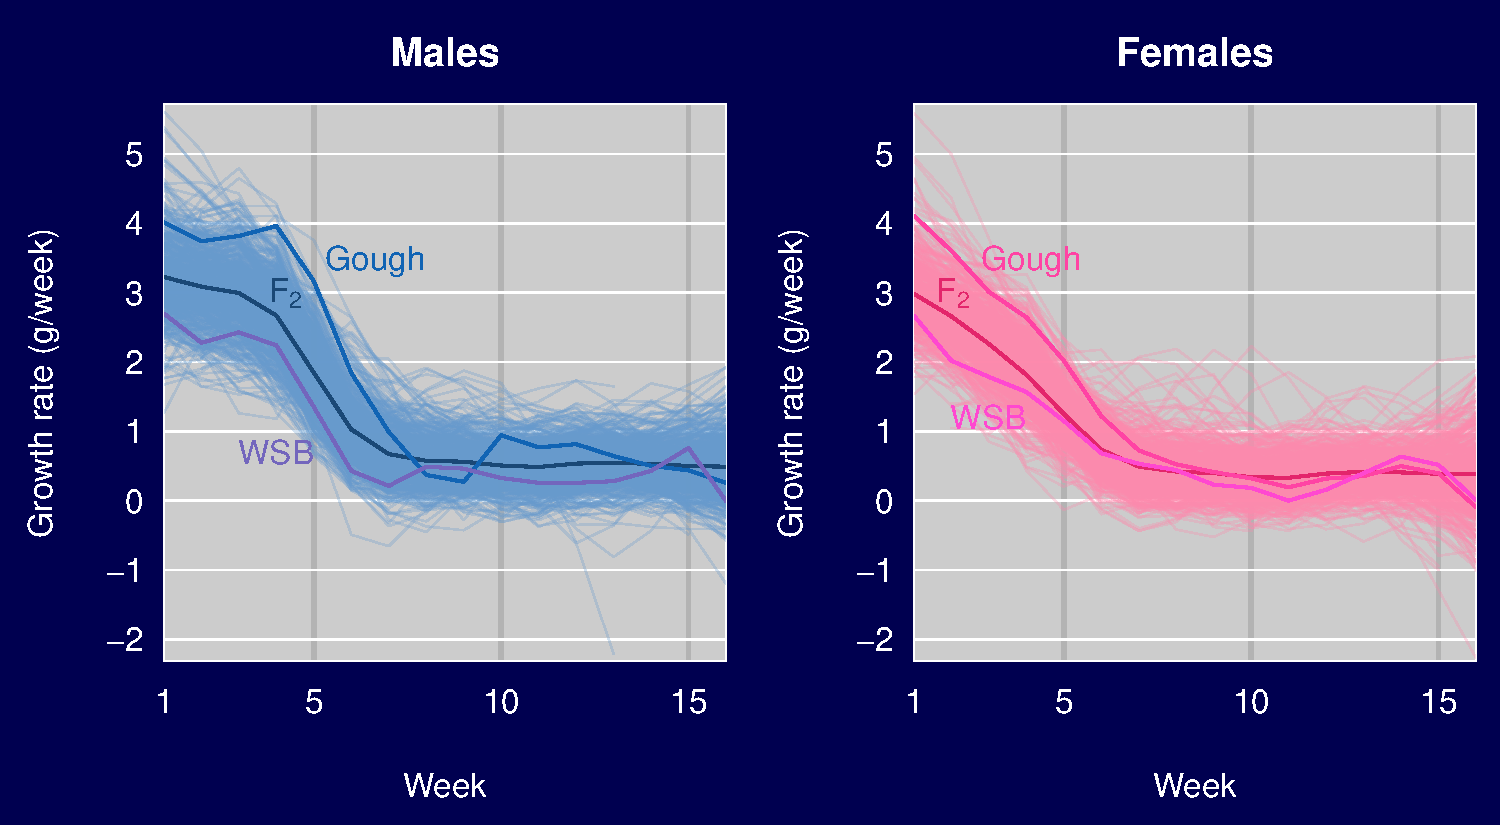
\includegraphics{Figs/rate3.pdf}}



\newpage

\headsize \color{myyellow}
\hfill \begin{minipage}{5.75in}
\centering
QTL scan for body weight
\end{minipage}

\vspace{5mm}

\centerline{\href{https://www.biostat.wisc.edu/~kbroman/presentations/CTC2014/iplot_bodyweight.html}{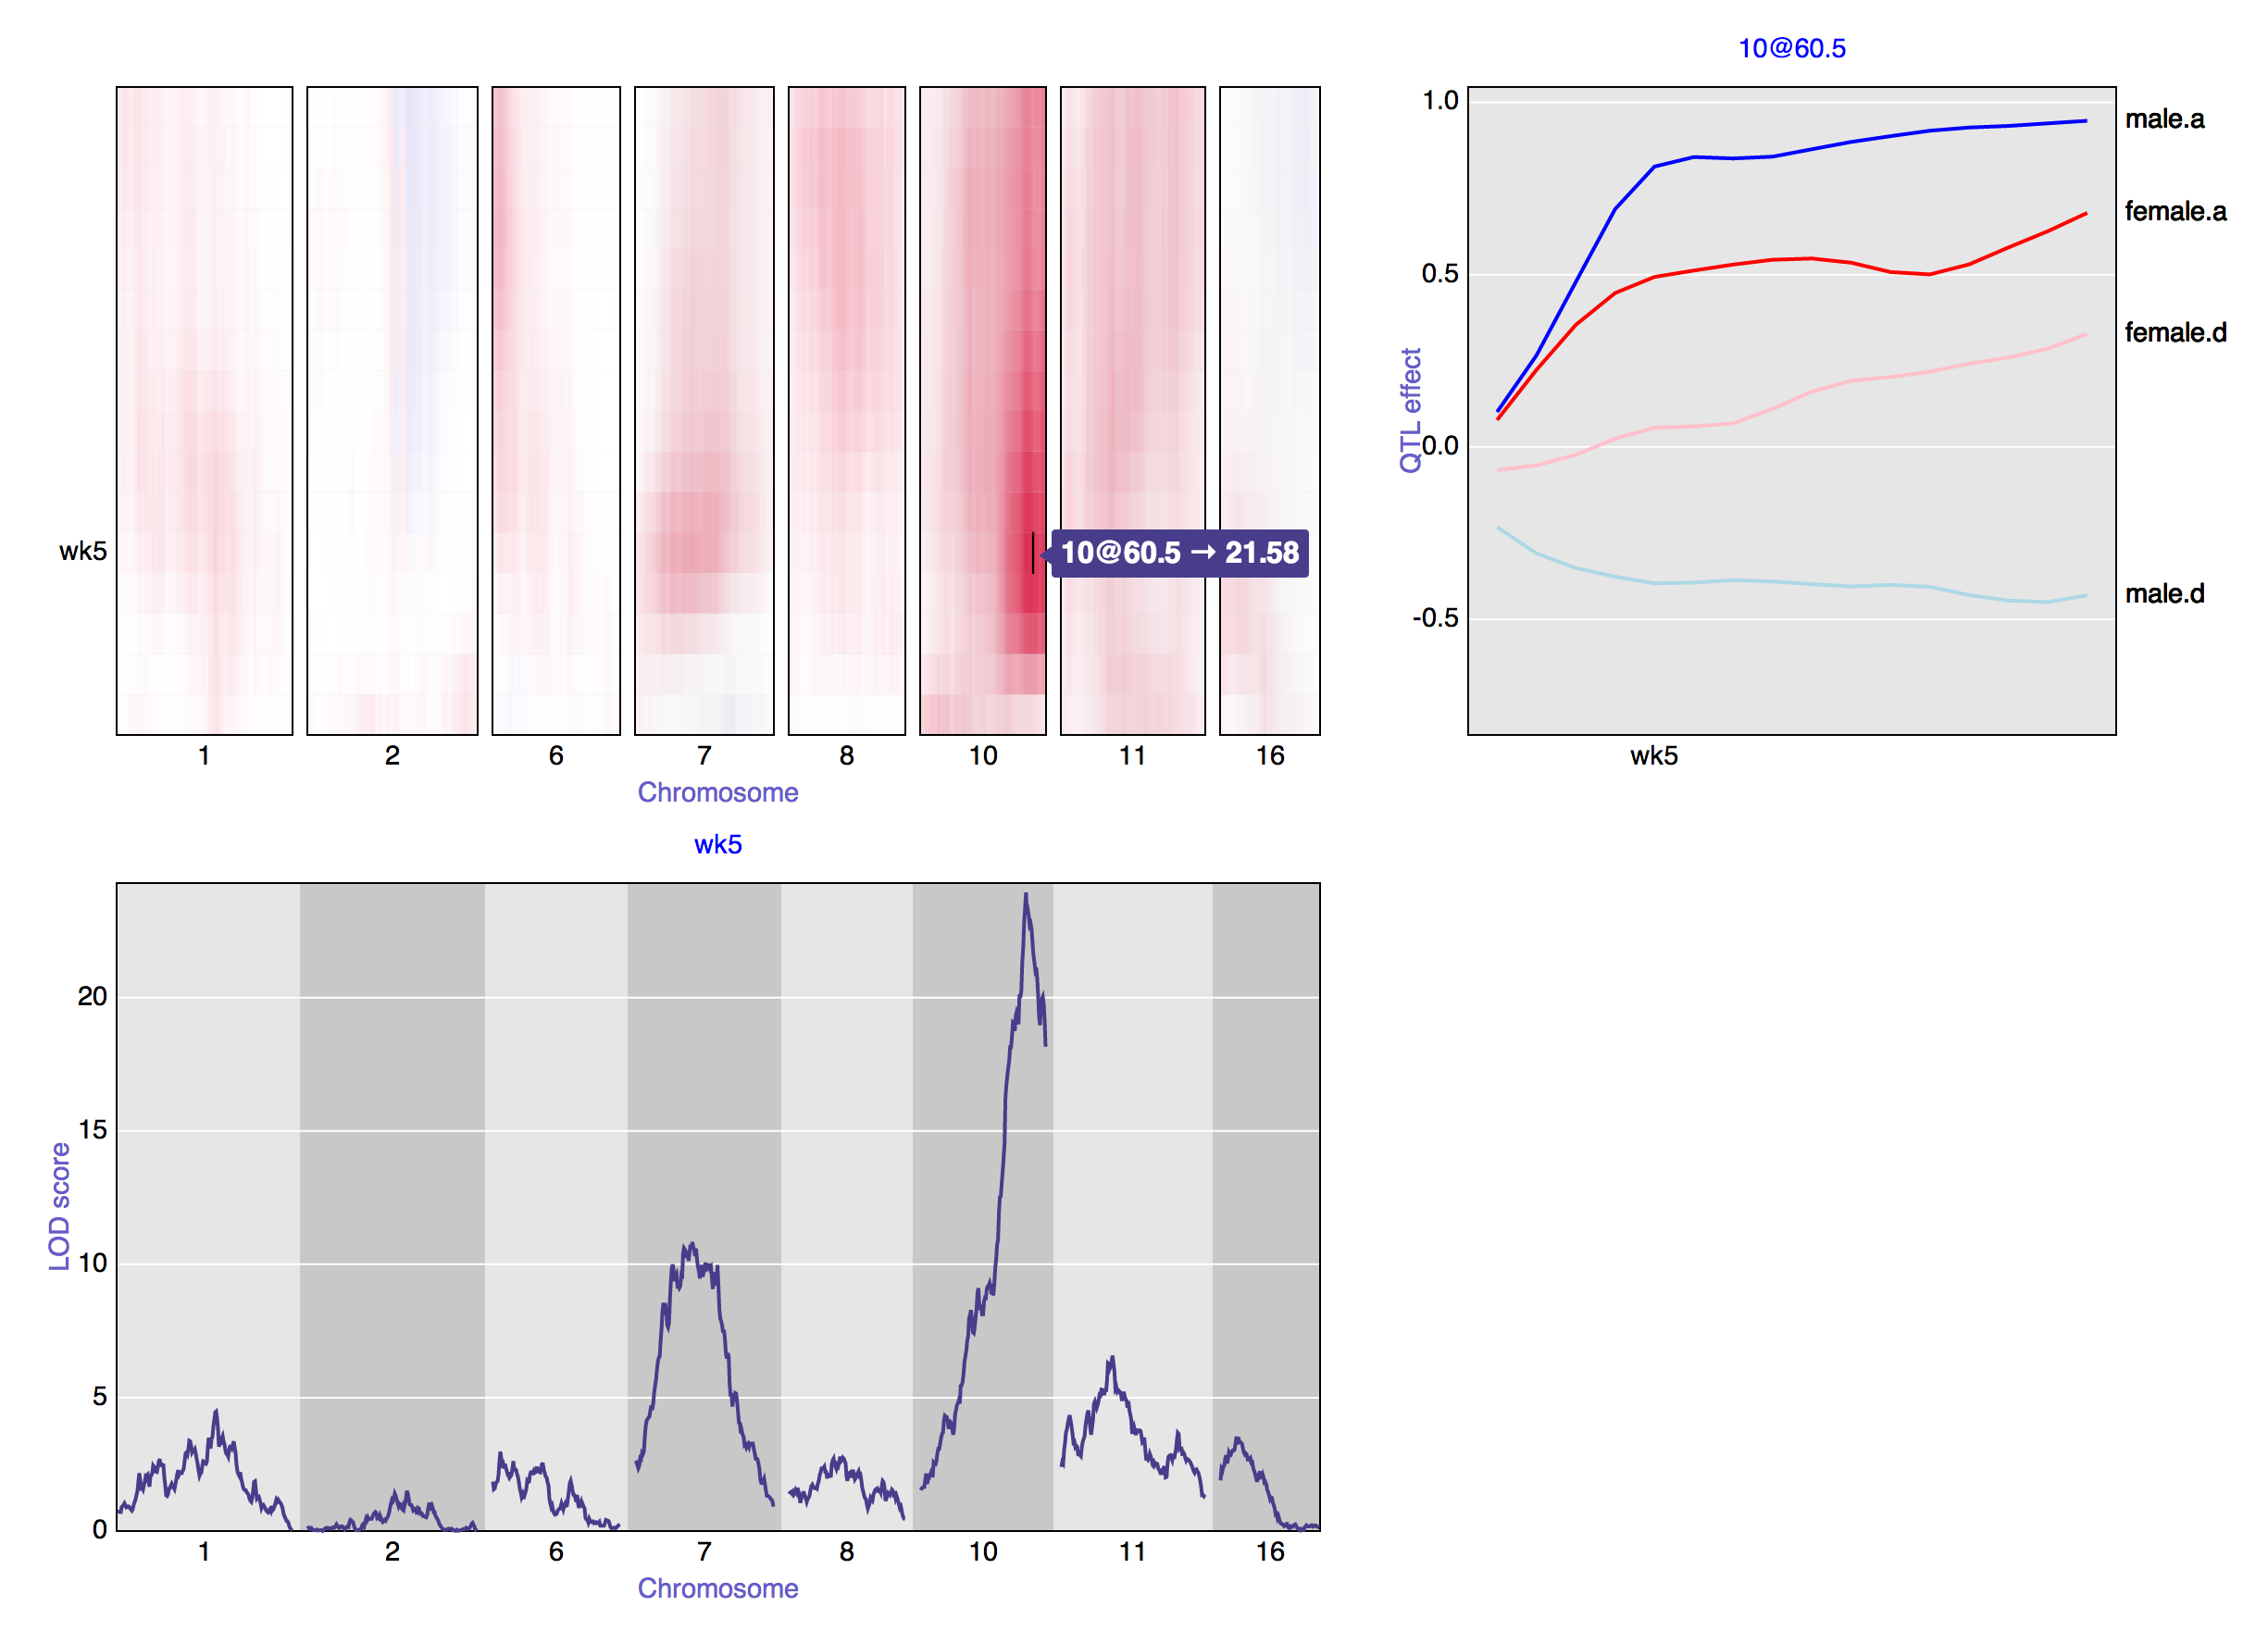
\includegraphics[height=0.9\textheight]{Figs/iplot_bodyweight.png}}}




\newpage

\headsize \color{myyellow}
\hfill \begin{minipage}{5.75in}
\centering
QTL scan for growth rate
\end{minipage}

\vspace{5mm}

\centerline{\href{https://www.biostat.wisc.edu/~kbroman/presentations/CTC2014/iplot_deriv_bodyweight.html}{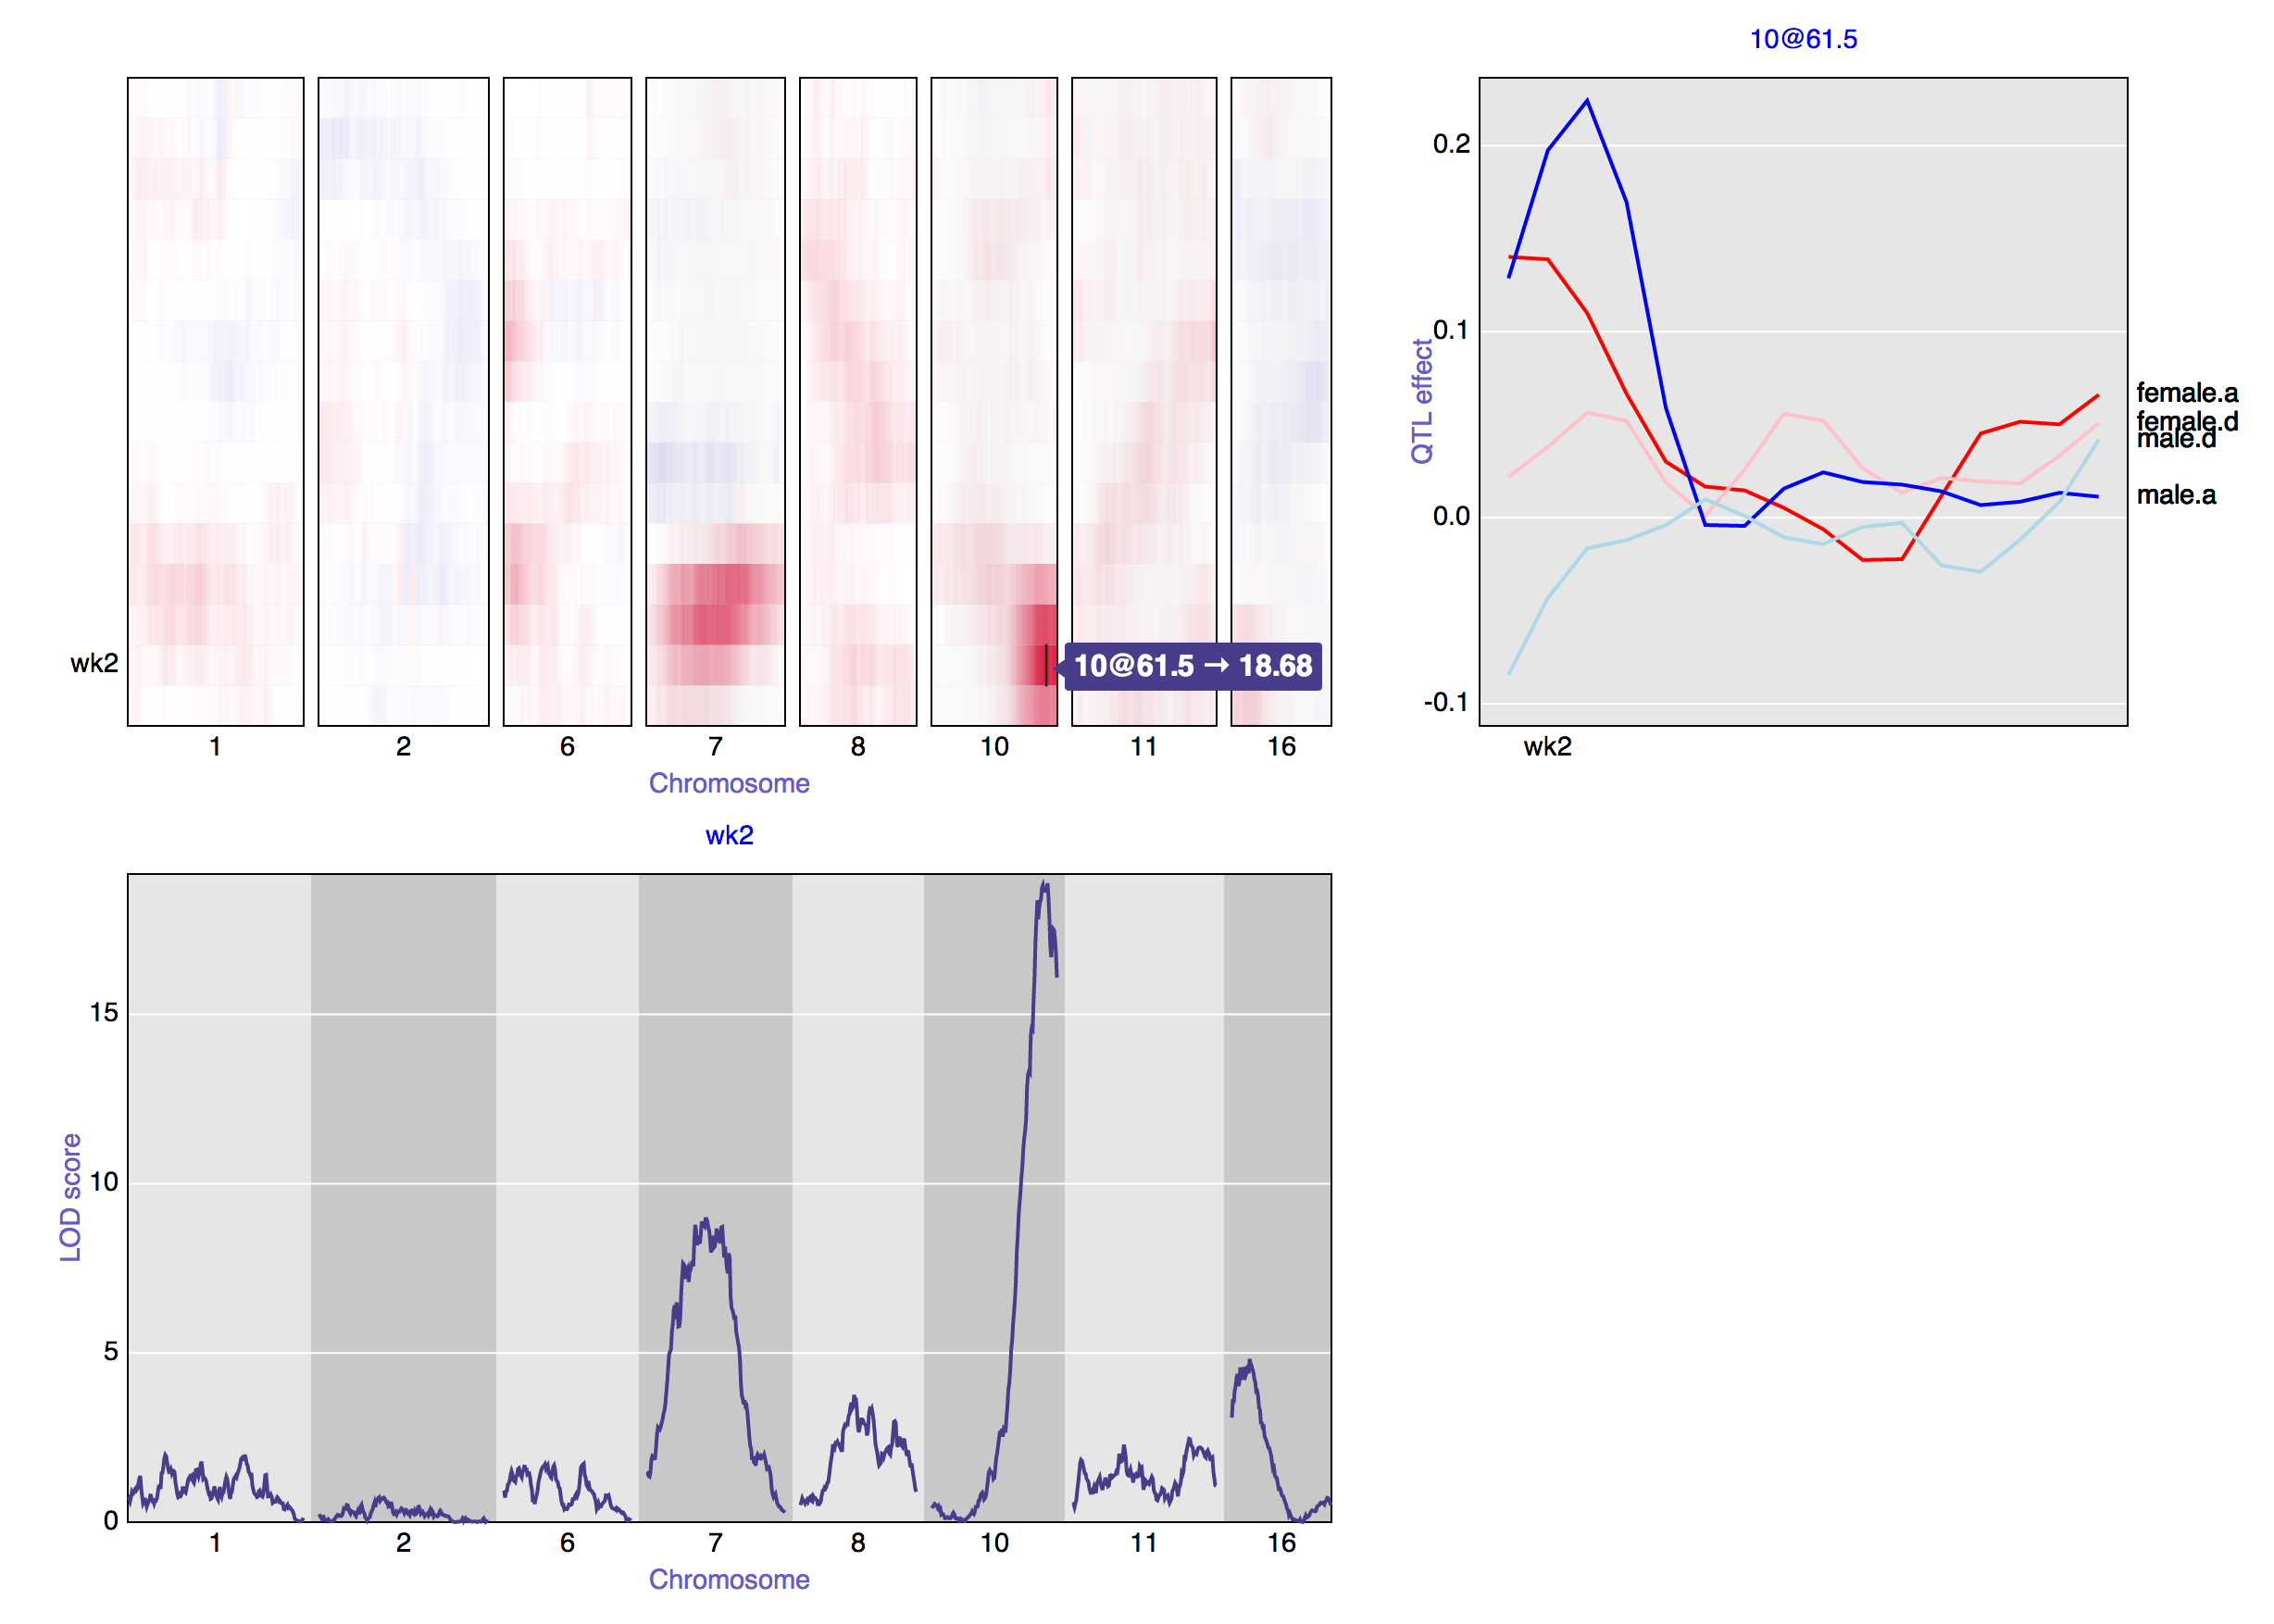
\includegraphics[height=0.9\textheight]{Figs/iplot_deriv_bodyweight.png}}}


\end{document}
